\chapter{Open Set Recognition}

Open set recognition with GAN \& OpenMax.

\section{GAN}

\subsection{GAN 原理笔记}

参考文献:\href{https://zhuanlan.zhihu.com/p/27295635}{GAN原理学习笔记-知乎}

传统的生成模型,如自编码机(Auto-Encoder),通常采取MSE作为Loss Function,这样的弊端是学习得到的Decoder模块性能不太令人满意。

\subsubsection{GAN原理}

首先,真实数据的分布已知,$P_{data}(x)$,我们需要做的就是生成一些也在这个分布内的图片,但无法直接利用这个分布。

刚才讨论过了,MSE的损失函数可能效果较差,改进办法是用交叉熵(Cross Entroy)来计算损失,从下面的推导可以看出,\textbf{交叉熵的最大化等价于KL散度的最小化}。KL散度衡量的是模型分布与真实数据分布之间的差异。

模型分布用$P_G$表示,数据分布用$P_{data}$表示。

\begin{align}
\hat{\theta} & = \argmax_{\theta} \prod_{i=0}^{m}P_G(y_i | x_i, \theta) \\
             & = \argmax_{\theta} \sum_{i=0}^{m} \log P_G(y_i | x_i, \theta) \notag \\
             & = \argmax_{\theta} E_{x \sim P_{data}} \log \log P_G(y_i | x_i, \theta)  \notag \\
             & = \argmax_{\theta} \int_{x} P_{data}(x) \log P_G(y_i | x_i, \theta)dx   - \int_{x} P_{data}(x) \log P_G(y_i | x_i, \theta) dx \\
             & = \argmin_{\theta} \int_{x}P_{data}(x) \log \frac{P_{data}(x)}{P_G(x; \theta)} dx \\
             & = \argmin_{\theta} KL\left( P_{data}(x), P_G(x; \theta)  \right)
\end{align}

其中,$m$表示从训练数据中采样的样本数。主要难理解的地方在于公式(6.2)中的后一项,由于这一项与$\theta$无关,所以加上之后也不会影响$\argmax_{\theta}$运算的取值。

\subsubsection{GAN公式}

\begin{equation}
\label{GAN:LossFunction0}
V(G, D) = E_{x \sim P_{data}}\left[ \log D(X) \right] + E_{x \sim P_{G}}\left[ 1-\log D(X) \right]
\end{equation}

优化目标是:
\begin{equation}
\label{GAN:ObjectFunction0}
G^{\star} = arg \min_G \max_D V(G, D)
\end{equation}

下面解释上面的两个式子。

$D$的作用是让这个式子尽可能的大。对于第一项,在输入$x$来自于真实数据时为了使$V$最大,$D(x)$应该接近于1;对于第二项,在输入$x$来自于$G$的生成时,则应该使$D(x)$尽可能的接近于0。

\subsubsection{训练过程}

根据公式\ref{GAN:LossFunction0}与\ref{GAN:ObjectFunction0},GAN的训练过程是$G$与$D$相互\textbf{迭代更新}的过程。具体如下:
\begin{figure}[!hbtp]
\centering
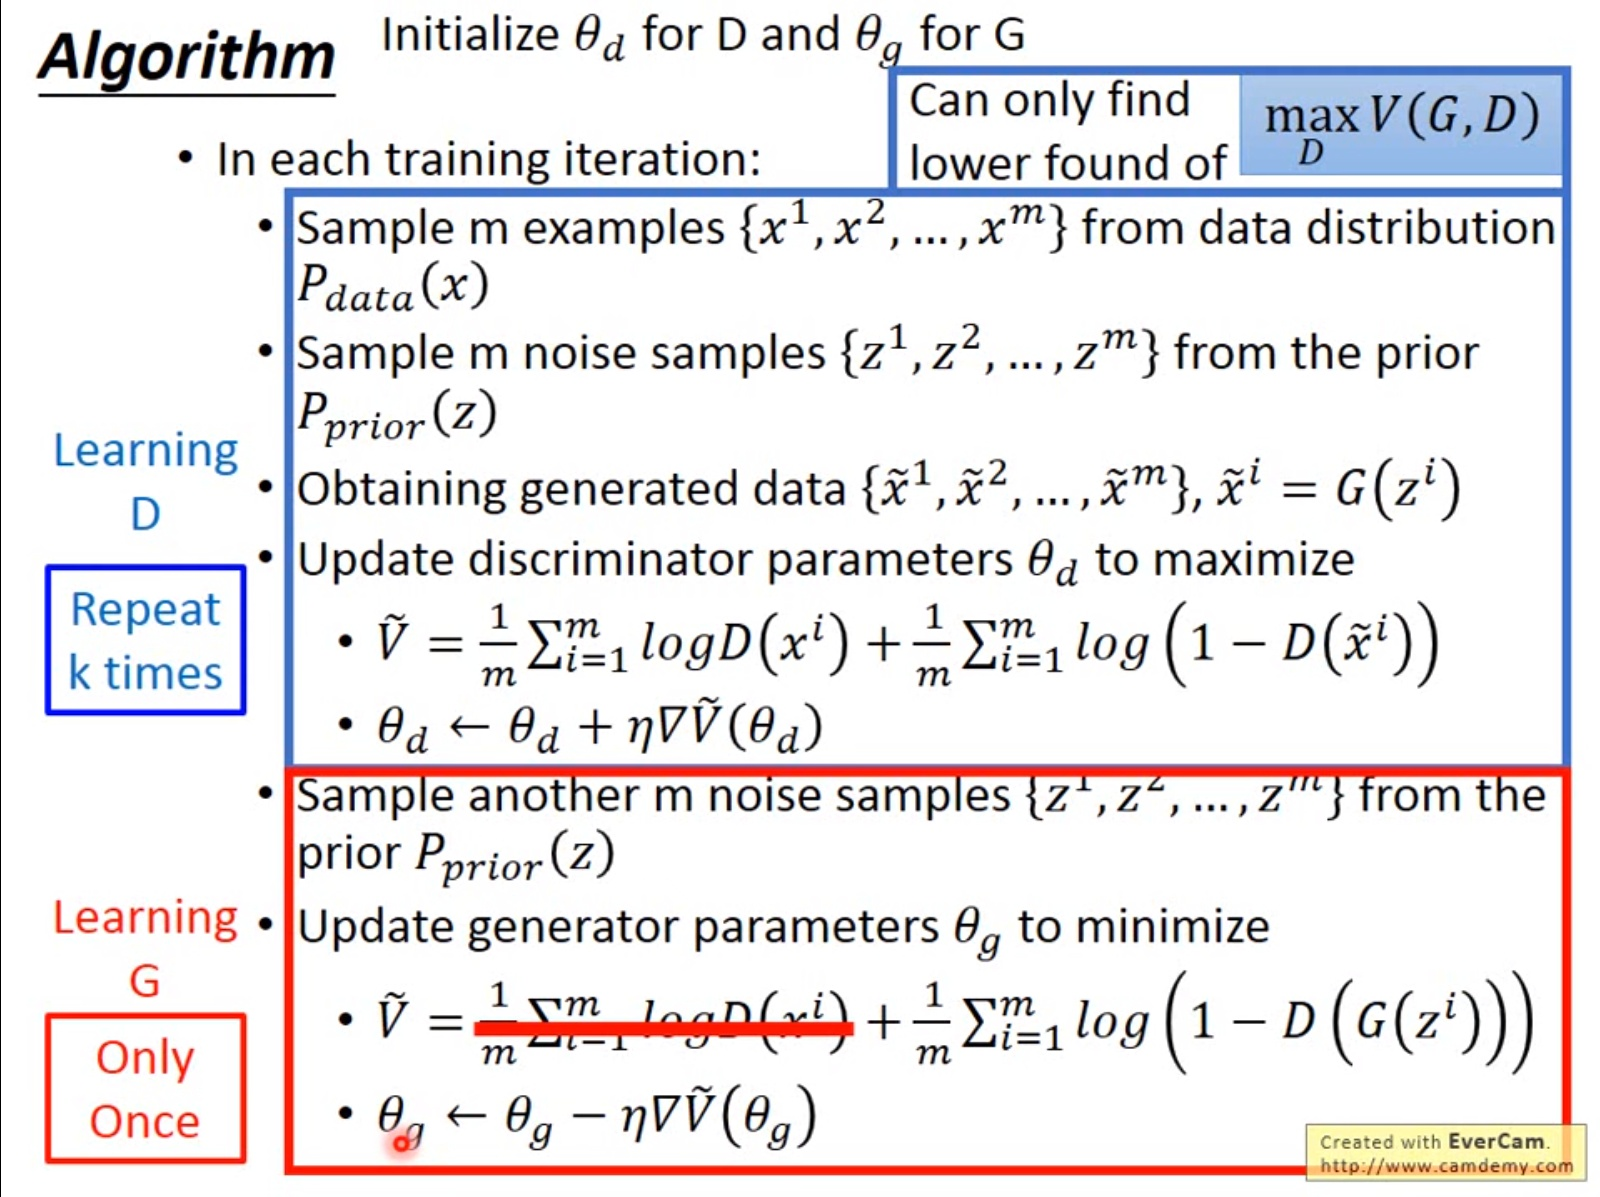
\includegraphics[width=0.75\textwidth]{OpenSetRecognition/GANTraining0.jpg}
\caption{GAN训练过程}
\label{GAN:Training0}
\end{figure}
注意,可能更新多次$D$次之后才更新一次$G$。



给定$G$,首先推导$D$的最优解。
\begin{align}
V(G, D) & = E_{x \sim P_{data}}\left[ \log D(X) \right] + E_{x \sim P_{G}}\left[ 1-\log D(X) \right] \notag \\
        & = \int_{x}P_{data}(x) \log D(x) dx + \int_x P_G \log (1-D(x)) dx \notag \\
        & = \int_x P_{data}(x) \log D(x) + P_G(x) \log(1-D(x)) dx \notag \\
\end{align}

在给定的$x$时,对上式中$D$的最大化,等价于:
\begin{displaymath}
\argmax_D \left[ \underset{a}{P_{data}(x)} \underset{D}{ \log D(x)} + \underset{b}{P_G(x)}(1 - \underset{D}{ \log D(x)}) \right]
\end{displaymath}

另
\begin{equation}
\label{GAN:ObjectFunction1}
f(D) = a \log D + b \log (1-D)
\end{equation}

对式\ref{GAN:ObjectFunction1}进行求导并另其为0得到最优$D$的表达式:
\begin{align}
D^{\star}(x) & = \frac{a}{a + b}   \notag \\
          & = \frac{P_{data}(x)}{P_{data}(x) + P_G(x)} \notag 
\end{align}

把上式关于$D$的最优解代入\ref{GAN:LossFunction0}可以得到以下公式:

\begin{align*}
\max_D V(G, D) & = V(G, D^{\star})    \\
               & = \int_{x}P_{data}(x) \log \frac{P_{data}(x)}{P_{data}(x) + P_G(x)} dx + \int_x P_G(x) \log  \frac{P_{G}(x)}{P_{data}(x) + P_G(x)} dx \\
               & = -2log2 + KL(P_{data}(x) \parallel \frac{P_{data}(x) + P_G(x)}{2}) + KL(P_{G}(x) \parallel \frac{P_{data}(x) + P_G(x)}{2}) \\
               & = -2 \log 2+ 2 JSD(P_{data}(x) \parallel P_G(x))
\end{align*}

其中, $JS$散度是$KL$散度的平滑版本,表示两个分部之间的差异。所以固定$G$时,$\max_D V(G, D)$表示两个分布之间的差异,最小值是$-2\log 2$,最大值是$0$。当$P_G(x) \equiv P_{data}(x)$, $G$是最优的。

\subsubsection{Loss Function中的两个小问题}

\begin{itemize}
\item 修改$G$的Loss Function

现有的$G$的Loss Function中的$\log (1- D(x)))$在$D(x)$趋近于0时,梯度非常小。所以在开始训练时,十分缓慢,一种改进办法是将其更改为:$\min_V = -\frac{1}{m}\sum_{i=1}^{m}\log(D(x^i))$


\item Mode Collapse

这是由于KL散度的不对称引起的,一种办法是将KL求解的顺序取反。即:$KL(P_{G} \parallel P_{data})$更改为$KL(P_{data} \parallel P_{G})$

\begin{displaymath}
KL(P_{data} \parallel P_{G}) = E_{x \sim P_{data}} \log P_G(x)
\end{displaymath}

\end{itemize}

{\color{red} Time: 2018.05.21}

\section{从头开始GAN}

参考文献:\href{https://zhuanlan.zhihu.com/p/27012520}{从头开始GAN 知乎}

\subsection{定义}

Ian Goodfellow自己的话说GAN\cite{Goodfellow2014GAN}:
\begin{quote}
The adversarial modeling framework is most straightforward to apply when the models are both
multilayer perceptrons. To learn the generator’s distribution pg over data $x$, we define a prior on
input noise variables $p_z(z)$, then represent a mapping to data space as $G(z; θ_g)$, where $G$ is a
differentiable function represented by a multilayer perceptron with parameters $θ_g$. We also define a
second multilayer perceptron $D(x; θ_d)$ that outputs a single scalar. $D(x)$ represents the probability
that $x$ came from the data rather than $p_g$. We train $D$ to maximize the probability of assigning the
correct label to both training examples and samples from $G$. We simultaneously train $G$ to minimize
$log(1 − D(G(z)))$.
\end{quote}

简单的说,GAN包含以下三个主要元素:
\begin{itemize}
\item 两个网络:一个生成网络$G$,一个判别网络$D$
\item 训练误差函数:
\begin{itemize}
\item G Net: $\log (1 - D(G(z)))$

希望$D(G(z))$趋近于1。

\item D Net: $-(\log D(x) + \log(1 - D(G(z))))$

D网络是一个二分类,希望真实数据的输出趋近于1,而生成数据的输出即$D(G(z))$趋近于0。

\end{itemize}
\item 数据输入:G Net的输入是随机噪声,D Net的输入是混合G的输出与真实数据样本的数据
\end{itemize}


值得注意的地方在于,训练D时,输入数据同时来自于真实数据$x$以及生成数据$G(z)$。且不用Cross Entropy的原因是,如果使用CE, 会使$D(G(z))$变为0,导致没有梯度,而GAN这里的做法是让$D(G(z))$收敛到0.5。

实际训练中,G Net使用了ReLU和Sigmoid,而D Net中使用了MaxOut和DropOut,并且修改了G Net的Loss Function,后一点可参考上一节。

但作者指出,此时的GAN不容易训练。

\subsection{DCGAN: Deep Convolution GAN}

DCGAN的几点改造:
\begin{itemize}
\item 去掉了G网络和D网络中的Pooling Layer
\item 在G网络和D网络中都是用BN
\item 去掉全连接的隐藏层
\item 在G网络中去除最后一层ReLU,改用Tanh
\item 在D网络中每一层使用LeakyReLU
\end{itemize}

G网络使用了4层反卷积,而D网络使用了4层卷积。基本上,G网络和D网络的结构正好反过来的。在使用DCGAN生成图像的研究线上,最新到了BEGAN(十个月以前),达到了以假乱真的效果。

\subsection{CGAN: Conditional Generative Adversarial Nets}

此时,输入不再仅是随机的噪声。就是在G网络的输入在z的基础上连接一个输入y,然后在D网络的输入在x的基础上也连接一个y:
\begin{figure}[!hbtp]
\centering
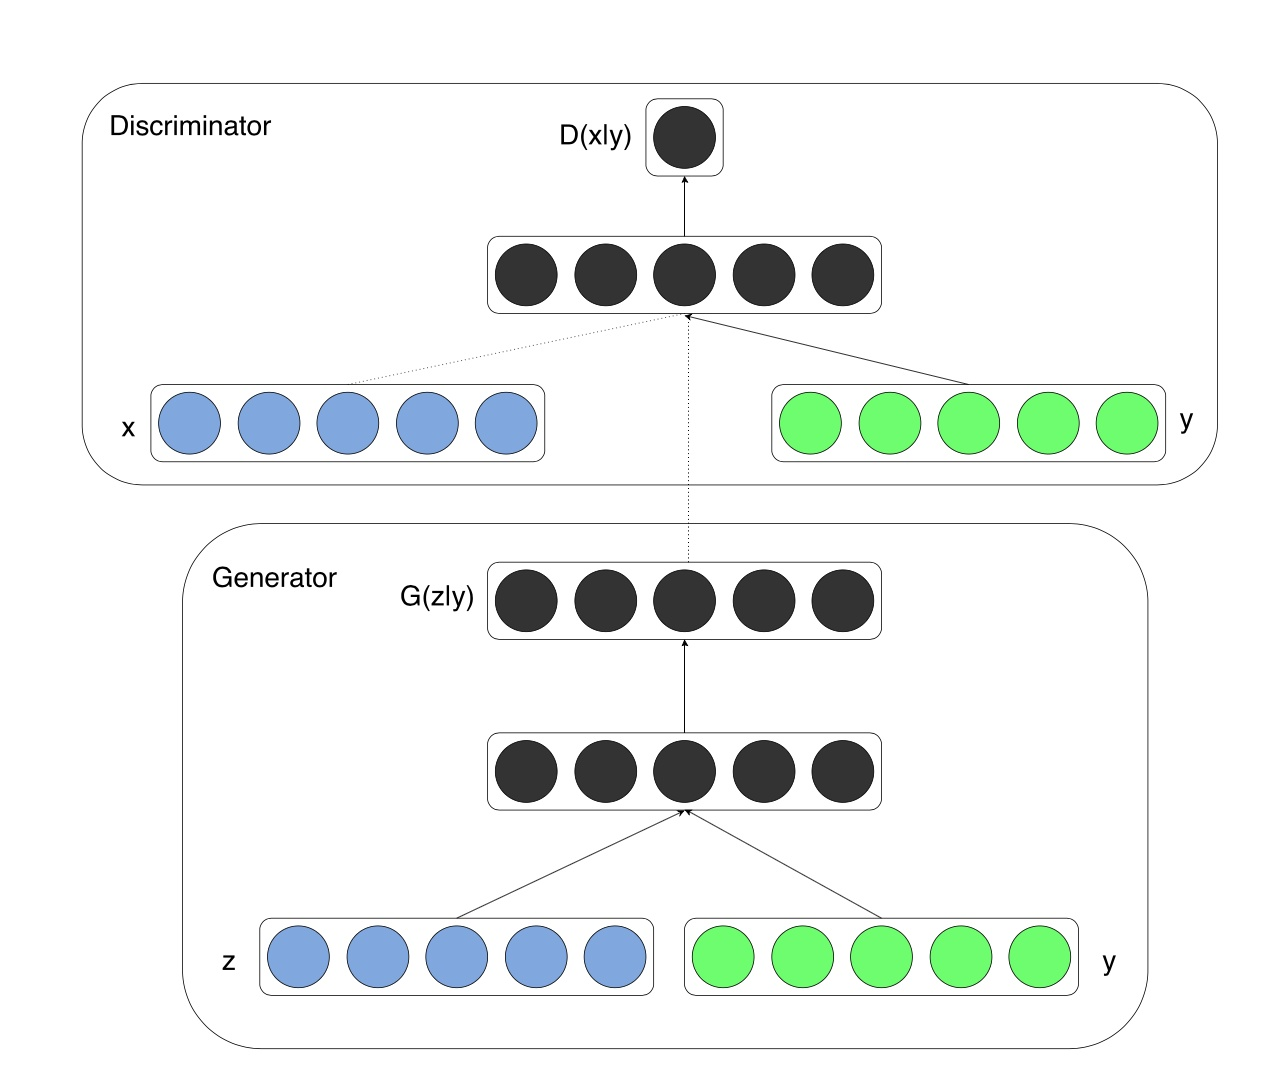
\includegraphics[width=0.85\textwidth]{OpenSetRecognition/CGAN0.jpg}
\caption{CGAN示意图,在G、N网络中新增了数据y}
\label{CGAN0}
\end{figure}

相应的目标函数变为:
\begin{displaymath}
arg \min_G \max_D V(D, G) = \mathbb{E}_{x \sim P_{data}}\left[ \log D(x | y) \right] + \mathbb{E}_{x \sim P_G} \left[ \log (1 - D(G(z | y))) \right]
\end{displaymath}

训练方式几乎就是不变的,但是从GAN的无监督变成了有监督。只是大家可以看到,这里和传统的图像分类这样的任务正好反过来了,图像分类是输入图片,然后对图像进行分类,而这里是输入分类,要反过来输出图像。显然后者要比前者难。


\subsection{InfoGAN}

在CGAN的基础上,将其变为无监督学习过程。要实现无监督的CGAN,意味着需要让神经网络不但通过学习提取了特征,还需要把特征表达出来。

怎么做呢?作者引入了信息论的知识,也就是mutual information互信息。作者的思路就是G网络的输入除了z之外同样类似CGAN输入一个c变量,这个变量一开始神经网络并不知道是什么含义,但是没关系,我们希望c与G网络输出的x之间的互信息最大化,也就是让神经网络自己去训练c与输出之间的关系。

Mutual Information在文章中的定义如下:
\begin{displaymath}
I(c, G(z, c)) = \mathbb{E}_{c \sim P(c), x \sim G(z, c)} \left[ \log Q(c|X) + H(c) \right]
\end{displaymath}

其中,$H$为熵运算。$Q$网络则是反过来基于X输出$c$。基于上式定义的$I$,则整个GAN的训练目标变为:
\begin{displaymath}
\min_G \max_D V(D, G) - \lambda I(c, G(z, c))
\end{displaymath}

相比于CGAN, InfoGAN又做了如下改变:
\begin{itemize}
\item D网络的输入只有$x$,不加$c$
\item Q网络和D网络共享同一个网络,只是到最后一层独立输出
\end{itemize}

\section{Generative Adversarial Nets}

参考文献:\cite{Goodfellow2014GAN}

{\color{red} \textbf{评语}: 需要重点关注,提出一个新的网络后,如何在数学上证明是可行的呢?}




\section{Towards Open Set Deep Networks}

引入了一种新型的新型的神经网络层结构,OpenMax,可以评估输入来自于一个未知类的概率。其中一个重要的组成部分是采用Meta-Recognition来对网络的Activation patterns进行处理。

比对SoftMax的结果进行Thresholding要好很多。(为什么会好?)

这是因为,实际使用中,即使输入是非常奇怪的,也就是说 "fooling" or "Rubbish" images时,网络也可能会在某一类上产生很高的输出概率,所以这时候通过设置Threshod的方式是不合适的。
\begin{quote}
They strongly
suggests that thresholding on uncertainty is not sufficient
to determine what is unknown.
\end{quote}

\subsection{Introduction \& Related Works}

In Sec. 3, we show that
extending deep networks to threshold SoftMax probabil-
ity improves open set recognition somewhat, but does not
resolve the issue of fooling images.

Thresholding可能会在某些时候会帮助Open Set Recognition,但对于Fooling images,结果可能比较差。

\section{Probability Models for Open Set Recognition}

本文的主要目的是,在限制Open Space Risk的分类算法中,使其能完成非线性多分类的功能。

此外,提出了Compact Abating Probability (CAP),也就是说,随着距离Known Data越来越远,即距离Open Space越来越近的时候,样本分类的概率会降低。

提出了具体的Weibull-calibrated SVM算法,该算法基于EVT原理进行Score Calibration,以及线性SVM来实现。

\textbf{本文的重点}:
\begin{itemize}
\item 提出了Compact abating probability (CAP)
\item 提出了Weibull-calibrate SVM (W-SVM):
\begin{itemize}
\item CAP
\item Statistic Extreme Value Theory (EVT)
\end{itemize}
\item 在Caltech 256 \& ImageNet上也有对比试验
\end{itemize}

\subsection{背景及相关工作}

















